\documentclass[12pt]{report}
\usepackage[utf8]{inputenc}
\usepackage[english, russian]{babel}
\usepackage{listings}
\usepackage{graphicx}
\usepackage{float}
\graphicspath{{imgs/}}
\usepackage{amsmath,amsfonts,amssymb,amsthm,mathtools} 
\usepackage{pgfplots}
\usepackage{filecontents}
\usepackage{indentfirst}
\usepackage{eucal}
\usepackage{enumitem}
\frenchspacing

\usepackage{indentfirst} % Красная строка

\usetikzlibrary{datavisualization}
\usetikzlibrary{datavisualization.formats.functions}

\usepackage{amsmath}
\usepackage{fixltx2e}
\usepackage{caption}


\definecolor{bluekeywords}{rgb}{0,0,1}
\definecolor{greencomments}{rgb}{0,0.5,0}
\definecolor{redstrings}{rgb}{0.64,0.08,0.08}
\definecolor{xmlcomments}{rgb}{0.5,0.5,0.5}
\definecolor{types}{rgb}{0.17,0.57,0.68}

\usepackage{listings}
\lstset{language=[Sharp]C,
	captionpos=t,
	numbers=left, %Nummerierung
	numberstyle=\small, % kleine Zeilennummern
	frame=single, % Oberhalb und unterhalb des Listings ist eine Linie
	stepnumber=1,                   
	numbersep=5pt,                
	showspaces=false,
	tabsize=2,
	showtabs=false,
	breaklines=true,
	showstringspaces=false,
	breakatwhitespace=true,
	escapeinside={(*@}{@*)},
	commentstyle=\color{greencomments},
	morekeywords={partial, var, value, get, set},
	keywordstyle=\color{bluekeywords},
	stringstyle=\color{redstrings},
	basicstyle=\ttfamily\small,
}

\usepackage[left=2cm,right=2cm, top=2cm,bottom=2cm,bindingoffset=0cm]{geometry}
% Для измененных титулов глав:
\usepackage{titlesec, blindtext, color} % подключаем нужные пакеты
\definecolor{gray75}{gray}{0.75} % определяем цвет
\newcommand{\hsp}{\hspace{20pt}} % длина линии в 20pt
% titleformat определяет стиль
\titleformat{\chapter}[hang]{\Huge\bfseries}{\thechapter\hsp\textcolor{gray75}{|}\hsp}{0pt}{\Huge\bfseries}

\usepackage{array}
\newcommand{\head}[2]{\multicolumn{1}{>{\centering\arraybackslash}p{#1}}{#2}}

% plot
\usepackage{pgfplots}
\usepackage{filecontents}
\usetikzlibrary{datavisualization}
\usetikzlibrary{datavisualization.formats.functions}

\begin{document}
%\def\chaptername{} % убирает "Глава"
\thispagestyle{empty}
\begin{titlepage}
	\noindent \begin{minipage}{0.15\textwidth}
		
\includegraphics[width=\linewidth]{b_logo}
	\end{minipage}
	\noindent\begin{minipage}{0.9\textwidth}\centering
		\textbf{Министерство науки и высшего образования Российской Федерации}\\
		\textbf{Федеральное государственное бюджетное образовательное учреждение высшего образования}\\
		\textbf{~~~«Московский государственный технический университет имени Н.Э.~Баумана}\\
		\textbf{(национальный исследовательский университет)»}\\
		\textbf{(МГТУ им. Н.Э.~Баумана)}
	\end{minipage}
	
	\noindent\rule{18cm}{3pt}
	\newline\newline
	\noindent ФАКУЛЬТЕТ $\underline{\text{«Информатика и системы управления»}}$ \newline\newline
	\noindent КАФЕДРА $\underline{\text{«Программное обеспечение ЭВМ и информационные технологии»}}$\newline\newline\newline\newline\newline\newline\newline\newline\newline\newline\newline
	
	
	\begin{center}
		\noindent\begin{minipage}{1.3\textwidth}\centering
			\Large\textbf{Отчет по лабораторной работе №5}\newline
			\textbf{по дисциплине "Анализ алгоритмов"}\newline\newline
		\end{minipage}
	\end{center}
	
	\noindent\textbf{Тема} $\underline{\text{Конвейерные вычисления}}$\newline\newline
	\noindent\textbf{Студент} $\underline{\text{Малышев И. А.}}$\newline\newline
	\noindent\textbf{Группа} $\underline{\text{ИУ7-51Б}}$\newline\newline
	\noindent\textbf{Оценка (баллы)} $\underline{\text{~~~~~~~~~~~~~~~~~~~~~~~~~~~}}$\newline\newline
	\noindent\textbf{Преподаватель: } $\underline{\text{Волкова Л. Л.}}$\newline\newline\newline
	
	\begin{center}
		\vfill
		Москва~---~\the\year
		~г.
	\end{center}
\end{titlepage}

\newpage
\renewcommand{\contentsname}{Содержание}
\setcounter{page}{2}
\tableofcontents

\newpage
\chapter*{Введение}
\addcontentsline{toc}{chapter}{Введение}

При обработке данных могут возникать ситуации, когда один набор данных необходимо обработать последовательно несколькими алгоритмами. В таком случае удобно использовать конвейерную обработку данных, что позволяет на каждой следующей <<линии>> конвейера использовать данные, полученные с предыдущего этапа. 

Помимо линейной конвейерной обработки данных, существуют параллельная конвейерная обработка данных. При таком подходе все линии работают с меньшим времени простоя, так как могут обрабатывать задачи независимо от других линий.

\textbf{Целью} данной лабораторной работы является изучение и реализация параллельной и линейной реализации конвейерной обработки данных.

В рамках выполнения работы необходимо решить следующие \textbf{задачи}:

\begin{itemize}
	\item изучить конвейерную обработку данных;
	\item реализовать систему конвейерных вычислений с количеством линий не меньше трёх;
	\item сравнить параллельную и линейную реализацию конвейерных вычислений;
	\item сделать выводы на основе проделанной работы.
\end{itemize}

\newpage
\chapter{Аналитическая часть}
В данной части будут рассмотрены главные принципы конвейерной обработки и параллельных вычислений.

\section{Общие сведения о конвейерной обработке}

\textbf{Конвейер} – машина непрерывного транспорта \cite{mednov}, предназначенная для перемещения сыпучих, кусковых или штучных грузов.

\textbf{Конвейерное производство} - система поточной организации производства на основе конвейера, при которой оно разделено на простейшие короткие операции, а перемещение деталей осуществляется автоматически. Это такая организация выполнения операций над объектами, при которой весь процесс воздействия разделяется на последовательность стадий с целью повышения производительности путём одновременного независимого выполнения операций над несколькими объектами, проходящими различные стадии. Конвейером также называют средство продвижения объектов между стадиями при такой организации\cite{wiki}. Появилось в 1914 году на производстве Модели-Т на заводе Генри Форда\cite{ford} и произвело революцию сначала в автомобилестроении, а потом и во всей промышленности.

В терминах программирования ленты конвейера представлены функциями, выполняющими над неким набором данных операции и предающие их на следующую ленту конвейера. Моделирование конвейерной обработки хорошо сочетается с технологией многопоточного программирования - под каждую ленту конвейера выделяется отдельный поток, все потоки работают в асинхронном режиме.

\section{Параллельное программирование}
\textbf{Параллельные вычисления} — способ организации компьютерных вычислений, при котором программы разрабатываются как набор взаимодействующих вычислительных процессов, работающих параллельно (одновременно). 

При использовании многопроцессорных вычислительных систем с общей памятью обычно предполагается, что имеющиеся в составе системы процессоры обладают равной производительностью, являются равноправными при доступе к общей памяти, и время доступа к памяти является одинаковым (при одновременном доступе нескольких процессоров к одному и тому же элементу памяти очередность и синхронизация доступа обеспечивается на аппаратном уровне). Многопроцессорные системы подобного типа обычно именуются симметричными мультипроцессорами (symmetric multiprocessors, SMP).

Перечисленному выше набору предположений удовлетворяют также активно развиваемые в последнее время многоядерные процессоры, в которых каждое ядро представляет практически независимо функциони рующее вычислительное устройство.

Обычный подход при организации вычислений для многопроцессорных вычислительных систем с общей памятью – создание новых параллельных методов на основе обычных последовательных программ, в которых или автоматически компилятором, или непосредственно программистом выделяются участки независимых друг от друга вычислений. Возможности автоматического анализа программ для порождения параллельных вычислений достаточно ограничены, и второй подход является преобладающим. При этом для разработки параллельных программ могут применяться как новые алгоритмические языки, ориентированные на параллельное программирование, так и уже имеющиеся языки, расширенные некоторым набором операторов для параллельных вычислений.

Широко используемый подход состоит и в применении тех или иных библиотек, обеспечивающих определенный программный интерфейс (application programming interface, API) для разработки параллельных программ. В рамках такого подхода наиболее известны Windows Thread API. Однако первый способ применим только для ОС семейства Microsoft Windows, а второй вариант API является достаточно трудоемким для использования и имеет низкоуровневый характер \cite{Barkalov}.

\subsection{Организация взаимодействия параллельных потоков}
Потоки исполняются в общем адресном пространстве параллельной программы. Как результат, взаимодействие параллельных потоков можно организовать через использование общих данных, являющихся доступными для всех потоков. Наиболее простая ситуация состоит в использовании общих данных только для чтения. В случае же, когда общие данные могут изменяться несколькими потоками, необходимы специальные усилия для организации правильного взаимодействия.

\section*{Вывод}
В данном разделе были рассмотрены основы конвейерной обработки, технология параллельного программирования и
организация взаимодействия параллельных потоков.


\newpage
\chapter{Конструкторская часть}
В данном разделе представлены схемы рассматриваемых алгоритмов.

\section{Разработка алгоритмов}
На рисунке 2.1 приведена схема организации конвейерных вычислений.

\begin{figure}[h]
	\centering
	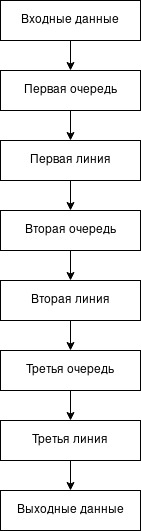
\includegraphics[scale=0.6]{imgs/scheme_lab05.jpg}
	\caption{Схема организации конвейерных вычислений.}
	\label{fig:mpr}
\end{figure}

\section*{Вывод}
В данном разделе была рассмотрена схема организации конвейерной обработки.


\newpage
\chapter{Технологическая часть}
Замеры времени были произведены на: Intel(R) Core(TM) i7-4790K, 4 ядра, 8 логических ядер.


\section{Средства реализации}
В качестве языка программирования был выбран C\# \cite{Microsoft} так как этот
язык поддерживает управление потоками на уровне ОС(незелёные потоки). В качестве среды разработки была выбрана Visual Studio. 
Время работы алгоритмов было замерено с помощью класса Stopwatch. Многопоточное программирование было
реализовано с помощью пространства имен System.Threading.


\section{Реализация алгоритмов}
В этой части будут рассмотрены листинги кода (листинг 3.1 - 3.3) реализованых алгоритмов.

\captionsetup{singlelinecheck = false, justification=raggedright}
\begin{lstlisting}[label=some-code,caption=Функция для запуска в потоке]
public void Run()
{
    state ret = state.ok;
    while(ret != state.finish)
    {
        ret = ProcessElement();
        if (ret == state.empty)
            Thread.Sleep(500);
    }
}
\end{lstlisting}

\newpage
\begin{lstlisting}[label=some-code,caption=Обработка элемента]
public state ProcessElement()
{
    Args el = null;
    lock(q)
    {
        if (q.Count > 0)
        {
            el = q.Dequeue();
        }
    }
    
    if (el != null)
    {
        if (el.IsLast())
        {
            if (nextLine != null)
                nextLine.AddElement(el);
            return state.finish;
        }
        conveyorAction(id, el, sleepTime);
        if (nextLine != null)
            nextLine.AddElement(el);
    }
    else
    {
        return state.empty;
    }

    return state.ok;
}
\end{lstlisting}


\begin{lstlisting}[label=some-code,caption=Добавление элемента в очередь]
public void AddElement(Args arg)
{
    lock (q)
    {
        q.Enqueue(arg);
    }
}
\end{lstlisting}
\captionsetup{singlelinecheck = false, justification=centering}

\section*{Вывод}
В данном разделе были рассмотрены основные сведения о средствах реализации и листинги кода реализованых алгоритмов.

\newpage
\chapter{Исследовательская часть}

\section{Сравнительный анализ на основе замеров времени}

Был проведен замер времени работы конвейерной и линейной обработки при разных временах обработки одной линии.
 
\begin{center}
\begin{tikzpicture}
\begin{axis}[
    	axis lines = left,
    	xlabel = {Максимальныая задержка(мс)},
    	ylabel = {Время (тики)},
	legend pos=north west,
	ymajorgrids=true
]


\addplot[color=yellow, mark=square] table[x index=0, y index= 1] {data/dataParallel.txt}; 
\addplot[color=orange, mark=square] table[x index=0, y index= 1] {data/dataLinear.txt}; 


\addlegendentry{Паралельный}
\addlegendentry{Линейный}

\end{axis}
\end{tikzpicture}

Pис. 4.1: Сравнение времени работы при разных значениях зедержек
\end{center}


На графиках видно, что конвейерная обработка с параллельными потоками в 2.5 раза быстрее, чем такая же линейная с захватом переменных.

\section{Тестирование}
Для тестирования был выведен лог операций в формате:
\begin{enumerate}
	\item id конвейера; 
	\item состояние;
	\item id элемента; 
	\item время на момент обработки.
\end{enumerate}

\begin{figure}[H]
	\center{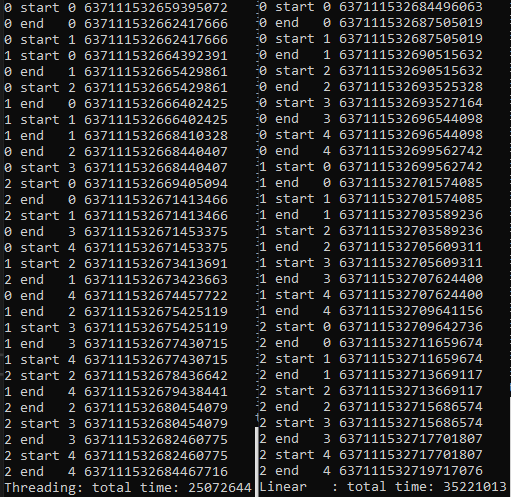
\includegraphics[scale = 0.7]{imgs/allDataTogether.png}}
	\caption{Лог работы конвейерной обработки}
	\label{fig:v_st}
\end{figure}



\section*{Вывод}
По результатам исследования конвейерную обработку нет смысла применять для задач, занимающих мало времени, т.к. в этом случае большая часть времени потратится на ожидание доступа к переменной, дополнительных проверок.
Тестирование показало, что конвейерная обработка реализована правильно.

\chapter*{Заключение}
\addcontentsline{toc}{chapter}{Заключение}
В ходе лабораторной работы были изучены возможности применения параллельных вычислений и конвейерной обработки и использован такой подход на практике. 

Был проведен эксперимент с разными значениями задержек, который показал, что если первый конвейер тормозит работу, то общее время работы системы линейно зависит от задержки первого конвейера. Данная зависимость распространяется не только на первый конвеер, т. е. конвеерные вычисления тормозятся из-за самого медленного конвеера. Также этот эксперимент показал, что конвейерную обработку нет смысла применять для задач, занимающих мало времени, т. к. в этом случае большая часть времени потратится на ожидание доступа к переменной, дополнительных проверок.

В рамках данной работы были решены следующие \textbf{задачи}:

\begin{itemize}
	\item изучена конвейерная обработка данных;
	\item реализована система конвейерных вычислений с количеством линий не меньше трёх;
	\item были сравнены параллельная и линейная реализация конвейерных вычислений;
	\item сделаны выводы на основе проделанной работы.
\end{itemize}

Поставленная цель была достигнута.

\newpage
\addcontentsline{toc}{chapter}{Список литературы}
\renewcommand\bibname{Список литературы}
\begin{thebibliography}{3}
	\bibitem{mednov} Меднов В.П., Бондаренко Е.П. Транспортные, распределительные и рабочие конвейеры. М., 1970.
	\bibitem{wiki} Конвейерное производство[Электронный ресурс] - режим доступа https:/ё/dic.academic.ru/dic.nsf/ruwiki/1526795
	\bibitem{ford} Koнвeйepный meтoд пpoизвoдcтвa Гeнpи Фopдa[Электронный ресурс] - режим доступа https://popecon.ru/305-konveiernyi-metod-proizvodstva-genri-forda.html
	\bibitem{Beloysov} И. В. Белоусов(2006), Матрицы и определители, учебное пособие по линейной алгебре, с. 1 - 16
	\bibitem{Barkalov} Константин Баркалов, Владимир Воеводин, Виктор Гергель. Intel Parallel Programming [Электронный ресурс], - режим доступа https://www.intuit.ru/studies/courses/4447/983/lecture/14925
	\bibitem{Beloysov} И. В. Белоусов(2006), Матрицы и определители, учебное пособие по линейной алгебре, с. 1 - 16
	\bibitem{Gall2012} Le Gall, F. (2012), "Faster algorithms for rectangular matrix multiplication", Proceedings of the 53rd Annual IEEE Symposium on Foundations of Computer Science (FOCS 2012), pp. 514–523
	%https://arxiv.org/pdf/1204.1111.pdf
	\bibitem{Barkalov} Константин Баркалов, Владимир Воеводин, Виктор Гергель. Intel Parallel Programming [Электронный ресурс], - режим доступа https://www.intuit.ru/studies/courses/4447/983/lecture/14925
	\bibitem{Microsoft} Руководство по языку C\#[Электронный ресурс], - режим доступа: https://docs.microsoft.com/ru-ru/dotnet/csharp/
\end{thebibliography}


\end{document}